\documentclass[12pt,a4paper,titlepage]{article}

\usepackage{graphicx}
\usepackage{amsmath}
\usepackage{amsthm}
%\usepackage{fullpage}
\usepackage{fancyheadings}
\usepackage{lastpage}
\usepackage{epsfig}
\usepackage{amsmath}
\usepackage{latexsym}
\usepackage{amssymb}
\usepackage{amstext}
\usepackage{fancyhdr}
\usepackage{array}
\usepackage{graphicx,picinpar,emlines2,epsf}



\begin{document}
\setlength{\parindent}{0pt} \setlength{\parskip}{2ex plus 0.5ex
minus 0.2ex}

\title{A Schedule for Lazy but Smart Ranchers}
\author{Team \# 1234}
\date{February 6, 2006}

\maketitle

\fancyhead{} \pagestyle{fancy} \lhead{Team \# 1234} \rhead{Page
\thepage\ of \pageref{LastPage}} \setlength{\headrulewidth}


\begin{abstract}
\setlength{\parindent}{0pt} \setlength{\parskip}{2ex plus 0.5ex
minus 0.2ex}

\noindent We present our three-stage model constructing process in
this paper. Firstly, we determine the number of sprinklers to use
by analyzing the energy and motion of water in the pipe and
examining the engineering parameters of sprinklers available in
the market.

Secondly, we build a model to determine how to layout the pipe
each time the equipment is reinstalled. This model leads to a
computer simulation of catch-can tests of the irrigation system
and an estimation of both distribution uniformity (DU) and
application efficiency of different schemes of where to move the
pipe. In this stage, DU is the most important factor we
considered. We also found a schedule in which one of the
sprinklers will be positioned out of the field in some moves, but
it results in higher DU (92.1\%) and actually saves more water.

In the final stage, we figure out two schedules to irrigate the
field. In one schedule, the field receives water evenly in time
during a cycle of irrigation (in our schedule, 4 days), while the
other one costs least labor force and time. In this stage, the
time and labor force required are the most important factors we
considered.

Our suggested solution, which is easy to implement, includes a
detailed timetable and the arrangement of the pipes. It costs 12.5
irrigation hours and 6 equipment resets in every cycle of 4 days
to irrigate the field with DU as high as 92.1\%.

\end{abstract}

\tableofcontents
\newpage

\section{Problem Review}
"Hand-move" irrigation system is one of various techniques for
irrigating a field. Pipes with sprinkler heads are put in place
across fields, and they are moved by hand at periodic intervals to
insure that the whole field receives an adequate amount of water.
This type of system is cheaper and easier to maintain but requires
a great deal of time and effort to move and set up the equipment
at regular intervals.

Use this system to irrigate an $80m\times30m$ field and work out a
scheme to minimize the amount of time required by a rancher to
maintain the irrigation system and maximize the uniformity. Given
a pipe set whose total length is $20m$, try to determine the
number of sprinklers and the spacing between sprinklers and find a
schedule to move the pipes, including where to move them. Each
pipe has a $10cm$ inner diameter with rotating spray nozzles that
have a 0.6$cm$ inner diameter. At the water source, the pressure
is 420kPa and has a flow rate of $150lpm$. No part of the field
should receive more than $0.75cmph$ of water, and each part of the
field should receive at least 2cm of water every 4 days.

\section{Assumptions and Definitions}
\begin{itemize}
\item The weather is assumed to be "fine" while the influence of
wind can be neglected.

\item The whole system is assumed to be "ideal" while evaporation, leaking and other ways of water loss can be neglected.


\item The water source can be moved and put at any position of the field. In practice, a tube can be used to transport water from the pump to the pipe set.

\item No mainline is assumed to exist so that all pipes join together and can be put at any position of the field.

\item The time for a rancher to uncouple, move and reinstall the pipe set is assumed to be half an hour.

\item The discharge of any sprinkler is assumed to be the same.

\item The manufacturer design pressure of sprinklers is assumed to be about 400kPa which is a most appropriate pressure in this problem and the type of rotating sprinkler is impact driven sprinkler (see details in Information & Analysis of Sprinklers section).

\item The diameter of the riser is assumed to be the same as that of the pipe.

\item The water pressures in pipes are assumed to be the same. In practice, there is a slight difference.

\end{itemize}

\begin{table}[!htb]
\centering \caption{Variables}
\begin{tabular}{lll}
\hline
\multicolumn{1}{c}{Variable} & Definition & \multicolumn{1}{c}{Units} \\
\hline
\multicolumn{1}{c}{p_{in}} & Water pressure in the pipe before a junction & \multicolumn{1}{c}{$kPa$} \\
\multicolumn{1}{c}{$p_{out}$} & Water pressure in the pipe after a junction & \multicolumn{1}{c}{$kPa$} \\
\multicolumn{1}{c}{$p_{up}$} & Water pressure at the sprinkler upon a junction & \multicolumn{1}{c}{$kPa$} \\
\multicolumn{1}{c}{$v_{in}$} & Water velocity in the pipe before a junction & \multicolumn{1}{c}{$m/s$} \\
\multicolumn{1}{c}{$v_{out}$} & Water velocity in the pipe after a junction & \multicolumn{1}{c}{$m/s$} \\
\multicolumn{1}{c}{$v_{up}$} & Water velocity at the sprinkler upon a junction & \multicolumn{1}{c}{$m/s$} \\
\multicolumn{1}{c}{$A_{in}$} & Section area in the pipe before a junction & \multicolumn{1}{c}{$cm^2$} \\
\multicolumn{1}{c}{$A_{out}$} & Section area in the pipe after a junction & \multicolumn{1}{c}{$cm^2$} \\
\multicolumn{1}{c}{$A_{up}$} & Section area at the sprinkler upon a junction & \multicolumn{1}{c}{$cm^2$} \\
\multicolumn{1}{c}{$h$} & Height of the sprinkler upon the pipe & \multicolumn{1}{c}{$m$} \\
\multicolumn{1}{c}{$t$} & Change in time & \multicolumn{1}{c}{$s$} \\
\multicolumn{1}{c}{$v_{source}$} & Water velocity of the water source & \multicolumn{1}{c}{$m/s$} \\
\multicolumn{1}{c}{$n$} & Number of sprinklers & \multicolumn{1}{c}{-} \\
\multicolumn{1}{c}{$distr(r)$} & Distribution function of precipitation profile & \multicolumn{1}{c}{-} \\
\multicolumn{1}{c}{$p$} & Precipitation rate & \multicolumn{1}{c}{-} \\
\multicolumn{1}{c}{$R$} & Sprinkling range & \multicolumn{1}{c}{$m$} \\
\multicolumn{1}{c}{$r$} & Distance from a sprinkler & \multicolumn{1}{c}{$m$} \\
\multicolumn{1}{c}{$r_i$} & Distance from the $i$th sprinkler & \multicolumn{1}{c}{$m$} \\
\multicolumn{1}{c}{$a$} & Obliquity of the precipitation profile & \multicolumn{1}{c}{$rad$} \\
\multicolumn{1}{c}{$pr(r)$} & Precipitation function of one sprinkler & \multicolumn{1}{c}{$cm/min$} \\
\multicolumn{1}{c}{$DU$} & Distribution Uniformity of an irrigation system & \multicolumn{1}{c}{-} \\
\hline
\end{tabular}
\end{table}

\begin{table}[!htb]
\centering \caption{Constants}
\begin{tabular}{lll}
\hline
\multicolumn{1}{c}{Variable} & \multicolumn{1}{c}{Definition} & \multicolumn{1}{c}{Value} \\
\hline
$ \rho$ & Density of water & $1.0kg/L$ \\
$g$ & Acceleration of gravity & $9.8m/s^2$ \\
\hline
\end{tabular}
\end{table}

\section{Problem Analysis}

Our goal is to determine the number of sprinklers and the spacing
between sprinklers and find a schedule to move the pipes,
including where to move them.

Our approach can be divided into three stages.

First, determine the number of sprinklers. In order to achieve the
goal, we figure out the pressure and velocity of water from each
sprinkler and then determine possible sprinkler number according
to some engineering data.

Second, determine where to put the pipes. We consider some major
factors such as sprinkling time, moving time and distribution
uniformity (DU) while DU is especially important for the purpose
of saving time. Since the pipe positions depend on the sprinkler
number and the precipitation profile, we just work out some
problem specific cases. However, our method can be used to solve
any practical cases.

Third, determine the schedule to move the pipes. Referring to the
water need of the field, a schedule is made to minimize the time
cost, which, obviously, is closely related to the positions of the
pipes to move.

\section{The Development of Models}

\subsection{Stage1: Water Pressure and Velocity}

\begin{figure}[!htb]
\centering
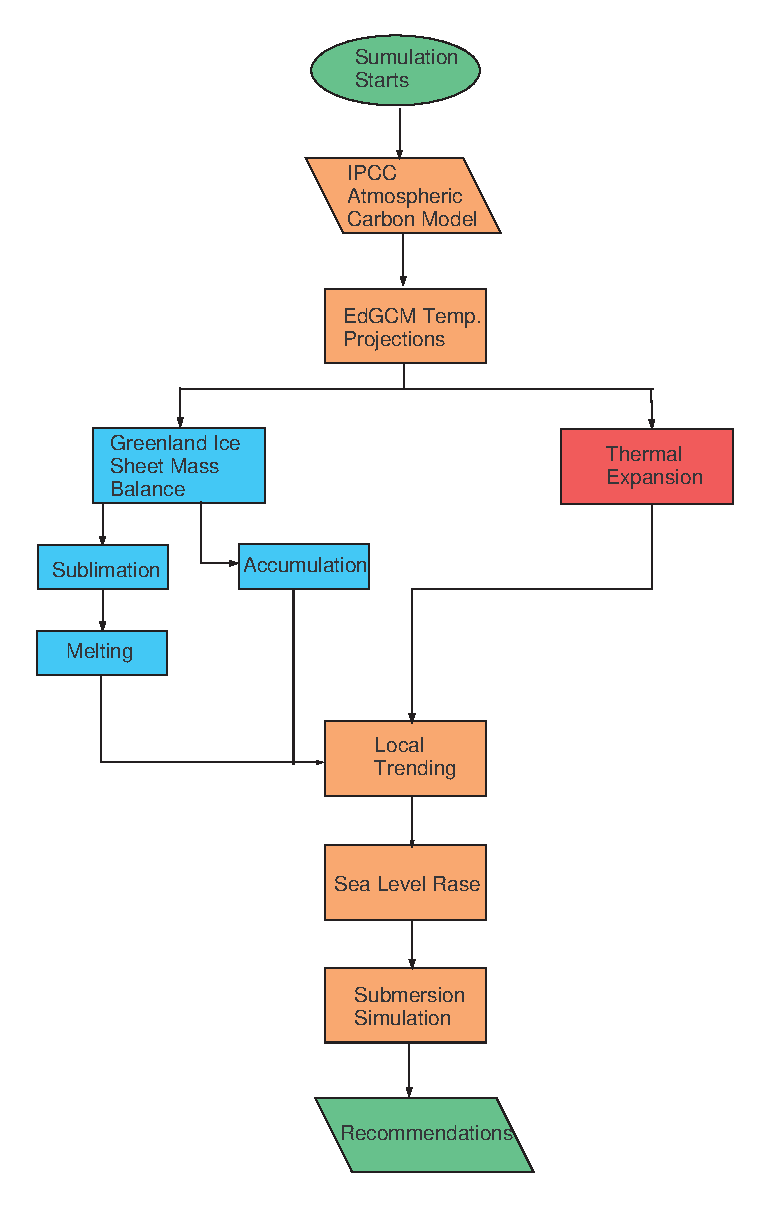
\includegraphics[width=0.8\textwidth]{fig01.eps}
\caption{\label{fig01} Overall sketch map with 4 sprinklers, 4
junctions numbered from 1 to 4.}
\end{figure}

The pressure of the shadow area is the same due to the last
assumption.

\begin{figure}[!htb]

\centering
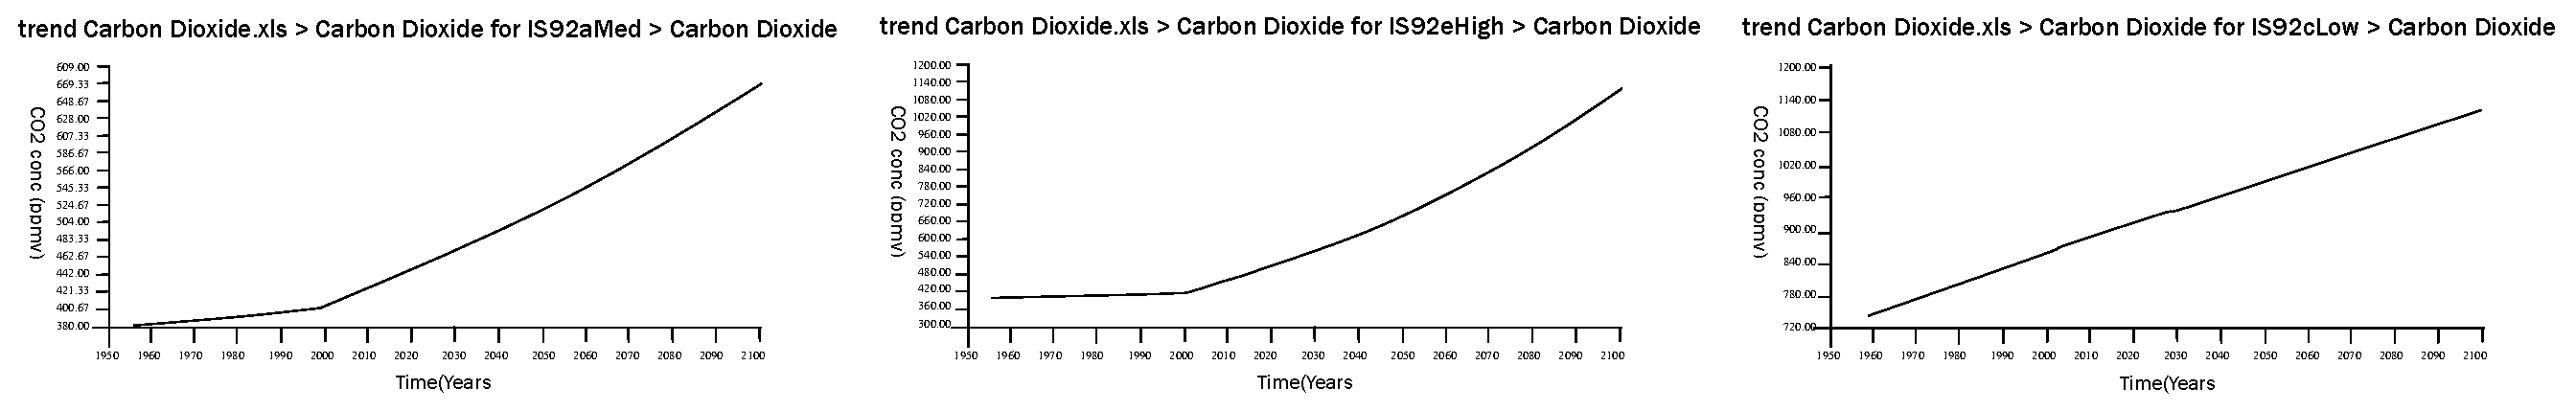
\includegraphics[width=0.8\textwidth]{fig02.eps}
\caption{\label{fig02} Sketch map at one junction.}
\end{figure}

We apply the law of conservation of energy to solve.

The work done by the forces is

\[
F_{in}s_{in}-F_{up}s_{up}-F_{out}s_{out}=p_{in}A_{in}v_{in}\Delta
t-p_{up}A_{up}v_{up}\Delta t-p_{out}A_{out}v_{out}\Delta t
\]

The decrease of potential energy is

\[
-mgh=-\rho gA_{up}v_{up}\Delta th
\]

The increase in kinetic energy is


\begin{eqnarray}
\frac{1}{2}mv_{up}^2+\frac{1}{2}mv_{out}^2-\frac{1}{2}mv_{in}^2=\frac{1}{2}\rho
A_{up}v_{up}\Delta tv_{up}^2+\frac{1}{2}\rho A_{out}v_{out}\Delta
tv_{out}^2\nonumber\\-\frac{1}{2}\rho A_{in}v_{in}\Delta
tv_{in}^2\nonumber
\end{eqnarray}

Putting these together, because of the law of conservation of
energy, gets

\begin{eqnarray}
p_{in}A_{in}v_{in}\Delta t-p_{up}A_{up}v_{up}\Delta
t-p_{out}A_{out}v_{out}\Delta t-\rho gA_{up}v_{up}\Delta th
\nonumber\\=\frac{1}{2}\rho A_{up}v_{up}\Delta
tv_{up}^2+\frac{1}{2}\rho A_{out}v_{out}\Delta
tv_{out}^2-\frac{1}{2}\rho A_{in}v_{in}\Delta tv_{in}^2
\end{eqnarray}

As the fluid is incompressible,

\begin{eqnarray}
A_{in}v_{in}=A_{up}v_{up}+A_{out}v_{out}
\end{eqnarray}

The diameters are all the same:

\begin{eqnarray}
A_{in}=A_{up}=A_{out}=\pi*(10cm/2)^2
\end{eqnarray}

According to assumptions, at every junction

\begin{eqnarray}
p_{in}=p_{out}=420kPa
\end{eqnarray}

\begin{eqnarray}
v_{up}=v_{source}/n
\end{eqnarray}

when

\[
v_{source}=\frac{150L/min}{\pi*(10cm/2)^2}=0.3183m/s
\]

Therefore, from (2),(3),(5), for the $i$th junction, its

\[
v_{in}=v_{source}(1-\frac{i-1}{n})
\]

and

\[
v_{out}=v_{source}(1-\frac{i}{n})
\]

Put (1),(2),(3),(4),(5) all together ,we can obtain $p_{up}$ at
every junctions.

\newpage

\begin{table}[!htb]
\centering \caption{Pressure at every sprinkler when $h=1m$ and
$n=4$.}
\begin{tabular}{ll}
\hline
\multicolumn{1}{c}{Junction No.} & \multicolumn{1}{c}{$P_{up}(Pa)$} \\
\hline
\multicolumn{1}{c}{1} & \multicolumn{1}{c}{410314} \\
\multicolumn{1}{c}{2} & \multicolumn{1}{c}{410257} \\
\multicolumn{1}{c}{3} & \multicolumn{1}{c}{410219} \\
\multicolumn{1}{c}{4} & \multicolumn{1}{c}{410200} \\
\hline
\end{tabular}
\end{table}

In fact, at the last (i.e. the $n$th) junction,

\[
v_{in}=v_{up}=\frac{v_{source}}{n}
\]

\[
v_{out}=0
\]

Put into (1), we can get

\[
p_{up}=p_{in}-\rho gh
\]


which means the pressure at the last sprinkler is independent of
$n$.

Commonly, $h$ is about $0.5m$ to $1.5m$, and even if assume
$h=1.5m$, the $v_{up}$ at the last junction will be $405300Pa$,
not far from $420kPa$. (if $h=0.5m$, the last $v_{up}$ will be
$415100Pa$)

From these equations, we can also know that the last $v_{up}$ is
the $v_{up}$ that differs most from $420KPa$, and the $v_{up}$ at
the first junction is the $v_{up}$ that close to $420kPa$ most
(and below $420kPa$),the values of $v_{up}$ are decreasing slowly
from junction 1 to $n$.

So we can come to this conclusion: all the values of $v_{up}$ at
every junction will be very close (all about $400kPa$, below
$420kPa$ and close to $420kPa$), no matter how many sprinklers
are. That's why we assume "design pressure of sprinklers is
assumed to be about $400 kPa$" in assumptions.

\newpage

\subsubsection{Information and Analysis of Sprinklers}

\begin{table}[!htb]
\centering
\caption{Data of sprinklers.[2] (Medium pressure
sprinklers have the best application uniformity.)}
\begin{tabular}{l|l|l|l}
\hline
\multicolumn{1}{c|}{Type} & \multicolumn{1}{c|}{Design Pressure} & \multicolumn{1}{c|}{Range} & \multicolumn{1}{c}{Discharge} \\
\multicolumn{1}{c|}{} & \multicolumn{1}{c|}{($kPa$)} & \multicolumn{1}{c|}{($m$)} & \multicolumn{1}{c}{($m^3/hour$)} \\
\hline
\multicolumn{1}{c|}{Low Pressure Sprinkler} & \multicolumn{1}{c|}{} & \multicolumn{1}{c|}{} & \multicolumn{1}{c}{} \\
\multicolumn{1}{c|}{(Low-Range Sprinkler)} & \multicolumn{1}{c|}{$<200$} & \multicolumn{1}{c|}{$<15.5$} & \multicolumn{1}{c}{$<2.5$} \\
\hline
\multicolumn{1}{c|}{Medium Pressure } & \multicolumn{1}{c|}{} & \multicolumn{1}{c|}{} & \multicolumn{1}{c}{} \\
\multicolumn{1}{c|}{Sprinkler} & \multicolumn{1}{c|}{} & \multicolumn{1}{c|}{} & \multicolumn{1}{c}{} \\
\multicolumn{1}{c|}{(Medium-Range } & \multicolumn{1}{c|}{200-500} & \multicolumn{1}{c|}{15.5-42} & \multicolumn{1}{c}{2.5-32} \\
\multicolumn{1}{c|}{Sprinkler)} & \multicolumn{1}{c|}{} & \multicolumn{1}{c|}{} & \multicolumn{1}{c}{} \\
\hline
\multicolumn{1}{c|}{High Pressure Sprinkler} & \multicolumn{1}{c|}{} & \multicolumn{1}{c|}{} & \multicolumn{1}{c}{} \\
\multicolumn{1}{c|}{(High-Range Sprinkler)} & \multicolumn{1}{c|}{$>500$} & \multicolumn{1}{c|}{$>42$} & \multicolumn{1}{c}{$>32$} \\
\hline
\multicolumn{1}{l}{} & \multicolumn{1}{l}{} & \multicolumn{1}{l}{} &  \\
\end{tabular}
\end{table}

There are 5 different types of rotating sprinklers among which the
impact driven sprinkler is the most widely used. In this article,
we assume that the rotating sprinkler is impact driven sprinkler.
Some rotating sprinklers have a sector mechanism that can wet
either a full circle or a sector, while rotating sprinklers
without sector mechanism can only wet a circle.

There are three main structure parameters of sprinklers: intake
line diameter, nozzle diameter, nozzle elevation angle.

An experiential formula is used to calculate the spraying range of
an impact driven sprinkler:

\[
R=1.70d^{0.487}h_p^{0.45}
\]

where $d$ is the nozzle diameter, $h_p$ is the operational
pressure head.

We have looked up a wide range of different models of impact
driven sprinklers, the following are the models with $6mm$ nozzle
diameter. The manufactory and some other information are omitted
here.[2]

\newpage


\begin{table}[!htb]
\centering \caption{Commonly available nozzle types whose diameter
is 6mm.}
\begin{tabular}{lllll}
\hline
Model & Nozzle diameter & Design pressure & Discharge & Range \\
 & ($mm$) & ($kPa$) & ($m^3/hour$) & ($m$) \\
\hline
PY$\neg_{1}$15 & 6 & 200 & 1.23 & 15.0 \\
 &  & 300 & 1.51 & 16.5 \\
\hline
PY$\neg_{1}$20 & 6 & 300 & 2.17 & 18.0 \\
 &  & 400 & 2.50 & 19.5 \\
\hline
PY$\neg_{1}$S20A & 6*4 & 300 & 2.99 & 17.5 \\
 &  & 400 & 3.41 & 19.0 \\
\hline
PY$_1$S20 & 6 & 300 & 2.22 & 18.0 \\
 &  & 400 & 2.53 & 19.5 \\
\hline
15PY$_2$22.5 & 6 & 350 & 2.40 & 17.0 \\
 &  & 400 & 2.56 & 17.5 \\
\hline
15PY$_2$30 & 6 & 350 & 2.40 & 18.0 \\
 &  & 400 & 2.56 & 18.5 \\
\hline
\end{tabular}

\end{table}

Sprinklers with higher manufacturer design pressure tend to have
larger wetted diameters. However, deviations from manufacturer's
recommended pressure may have the opposite effect (increase in
pressure, decrease in diameter), and uniformity will probably be
compromised.

The following picture shows typical precipitation distribution of
one sprinkler in low, correct, and high sprinkler pressure.


\begin{figure}[!htb]
\centering
\includegraphics[width=0.4\textwidth]{fig03.eps}
\caption{\label{fig03} Relation between pressure and precipitation
distribution.[2] (a) Pressure is too low (b) Pressure is ok (c)
Pressure is too high }
\end{figure}

In practice, people use catch-can data to generate precipitation
profile of a "hand move" irrigation system. That is to put
catch-cans evenly in the field, and, after irrigation, the
precipitation profile can be portrayed by the amounts of water
contained in each catch-can (Figure 4).[3]

\begin{figure}[!htb]
\centering
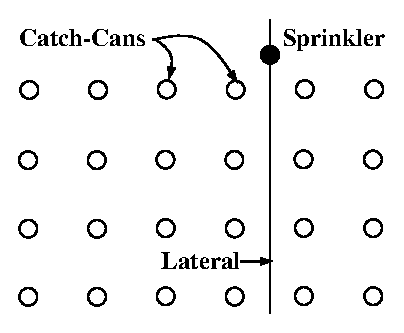
\includegraphics[width=0.4\textwidth]{fig04.eps}
\caption{\label{fig04} Catch-can test.[3] }
\end{figure}

One measure of how uniformly the water is applied to the field is
Distribution Uniformity (DU), which is defined as:[3]

\[
DU=\frac{\textit{average\_precipitation\_rate\_of\_low\_quarter}}{\textit{average\_precipitation\_rate}}\times100\%
(*)
\]


Usually, $DUs$ of less than 70\% are considered poor, $DUs$ of 70
- 90\% are good, and $DUs$ greater than 90\% are excellent. In
short, bad DU means that either too much water is applied, costing
unnecessary expense, or too little water is applied, causing
stress to crops. There must be good DU before there can be good
irrigation efficiency.[4]

To simplify our calculation, we approximate the precipitation
profile of a single sprinkler (in Figure 3(b)) to a function:
$distr(r)$, which means the relative precipitation rate in the
position with a distance $r$ from the sprinkler (Figure 5).

\begin{figure}[!htb]
\centering
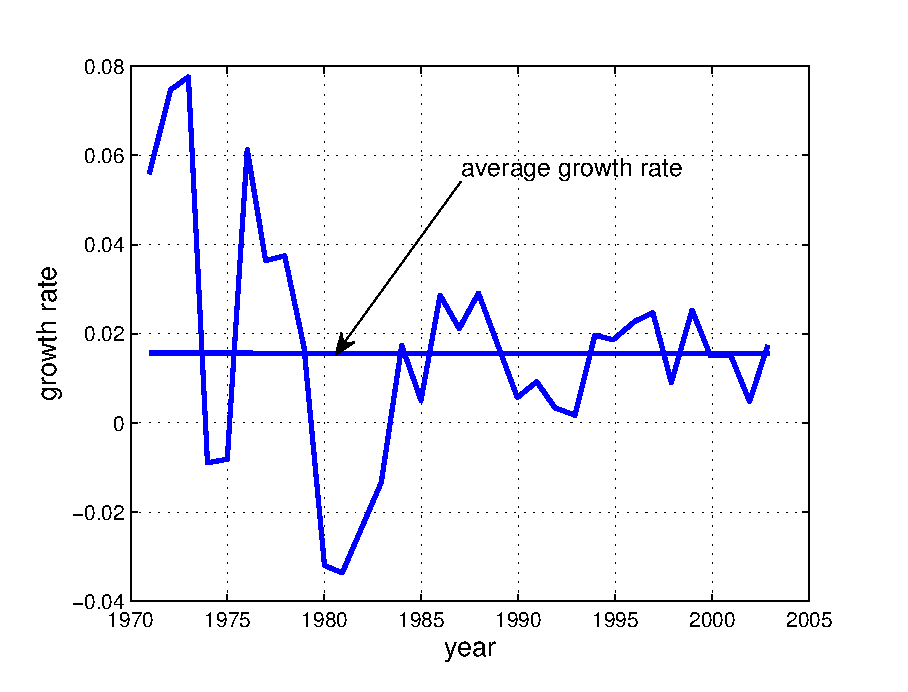
\includegraphics[width=0.6\textwidth]{fig05.eps}
\caption{\label{fig05} The precipitation rate plotted vs. the
distance to the sprinkler.}
\end{figure}

In this problem's case, surely we should use medium pressure
sprinklers (see Table 4).And In Table 5, for those sprinklers with
a $6mm$-diameter nozzle and working at $400kPa$ (as we assumed),
their discharge is $2.5-3.5m^3/hour$ and spraying range is 18.5,19
or $19.5m$. From now on, we'll use $19m$ as the range of
sprinklers concerned.

Note the discharge of the source is

\[
150L/min=9m^3/hour,
\]

thus, to fit every sprinkler's actual discharge to the design
discharge, the number of sprinklers we'll install should be 3 or
4. It is because $9/3=3$ or $9/4=2.25$, which is close to or
within the range of the $2.5-3.5m^3/hour$.

\subsection{Stage2: Scheduling the Irrigation}

Actually, a schedule to move the pipes includes both where and in
how long an interval to move them. For the previous one, we just
imagine a fixed irrigation system consisting of several $20m$
pipes. If the system can nicely, i.e. with high Distribution
Uniformity (DU), meet the needs of the crops, then the way of
moving the pipe in the problem is just to move it from one pipe's
position to another in the system. So, we'll determine where to
move the pipe by laying out a system of several 20m pipes, and
then decide for how long we should water the field before making a
next move. First, we use a simulation of catch-can analysis to
choose a layout with a high DU.

\subsubsection{Catch-can Analysis}

Since the water sprayed by a particular sprinkler has a determined
distribution: $distr(r)$, as we've already defined, we use the
following method to simulate the catch-can test.

For rectangular spacing (Figure 6 Left), we consider the
rectangular region between four adjacent sprinklers. In our
simulation, we pick 900 positions evenly distributed in the
region. For each position, we calculate its relative precipitation
rate $p$:

\[
p=\sum_idistr(r_i)
\]

$r_i$ is the distance from the position to a sprinkler considered.
Thus , for the $i$th position, we got pi,($1\leq i\leq900$). With
Equation (*), we then calculate the DU of this irrigation system.

\begin{figure}[!htb]
\centering
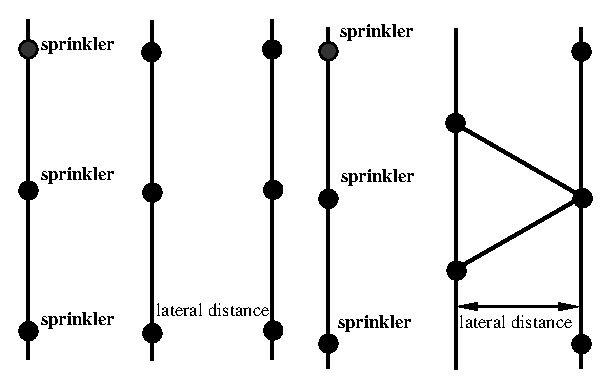
\includegraphics[width=0.6\textwidth]{fig06.eps}
\caption{\label{fig06} Left: Rectangular spacing; Right:
Triangular spacing.}
\end{figure}

As we've already deduced, the number of the sprinklers should be 3
or 4, thus the sprinkler distance will be $10m$ ($20m/(3-1)$) or
$6.67m$ ($20m/(4-1)$)\footnote{That the sprinkler distance is
evenly distributed along the pipe is because that it will have a
higher DU and it is easy to operate.}. So the DU is a function of
the lateral distance. And this can also be applied for triangular
spacing (Figure 6 Right). After the simulation, we get:

\begin{figure}[!htb]
\centering
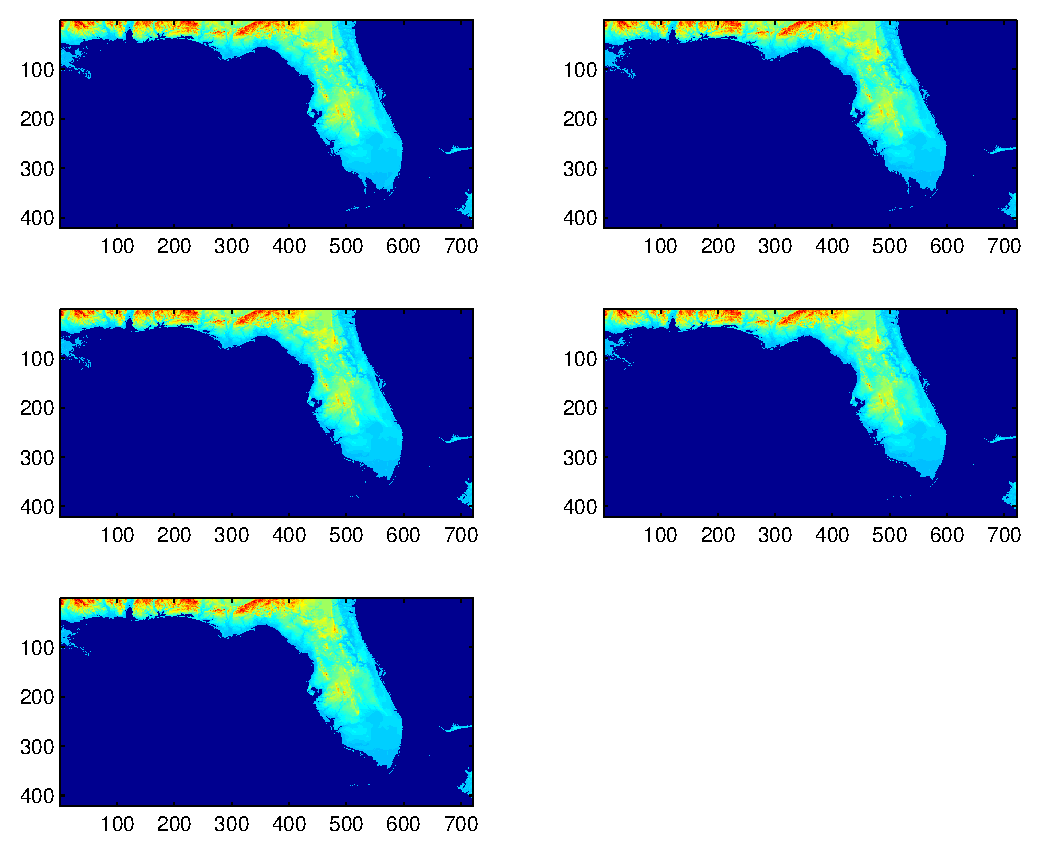
\includegraphics[width=0.8\textwidth]{fig07.eps} \caption{\label{fig07} $DU$ plotted vs.
lateral distance, in 4 different situations.}
\end{figure}

The simulation shows that when lateral distance $\leq 20$, $DU$ is
acceptable ($\geq 90\%$), regardless of the spacing and whether
the sprinkler distance is $6.67m$ or $10m$. But since larger
lateral distance will result in smaller amount of time required to
irrigate the field (the number of moves to make will be less), we
pick $20m$ as the lateral distance. Figure 8 and Figure 9 show the
precipitation profile for the irrigation systems with sprinkler
distance $10m$ and lateral distance $20m$.

\begin{figure}[!htb]
\centering
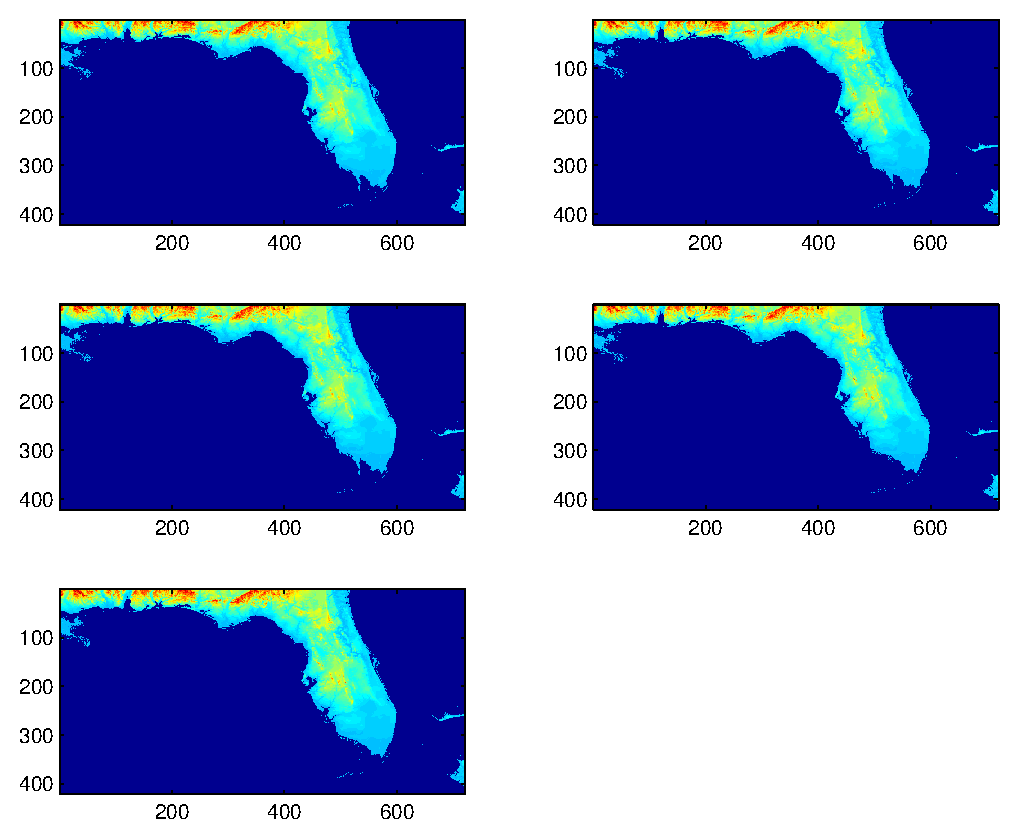
\includegraphics[width=0.8\textwidth]{fig08.eps} \caption{\label{fig08} Left: Precipitation profile for rectangular spacing with sprinkler distance $10m$ and lateral distance $20m$; right: the 3D form of the precipitation profile.}
\end{figure}


\[
 DU=98.1\%
\]

\begin{figure}[!htb]
\centering
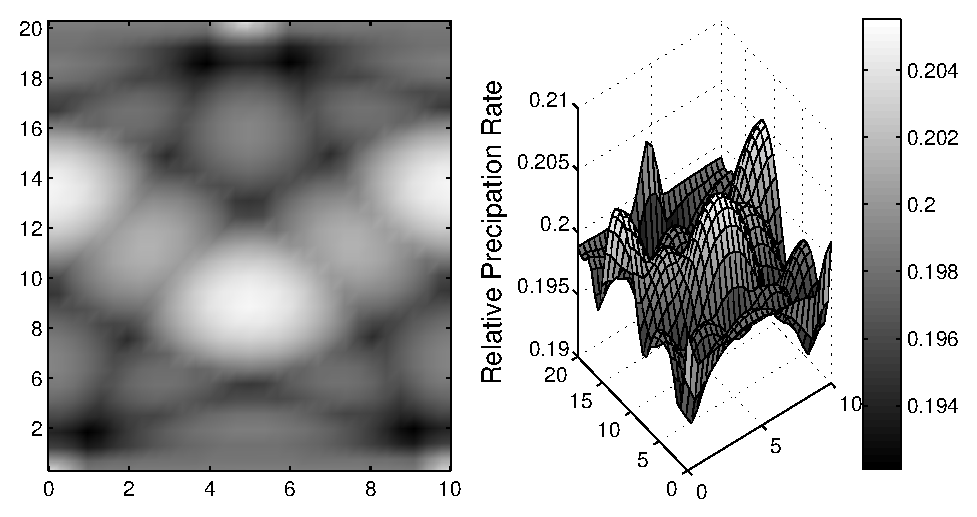
\includegraphics[width=0.8\textwidth]{fig09.eps} \caption{\label{fig09} Left: Precipitation profile for triangular spacing with sprinkler distance $10m$ and lateral distance $20m$; right: the 3D form of the precipitation profile. }
\end{figure}

\[
 DU=98.7\%.
\]

Considering that the field ($30m\times80m$) is not relatively
large enough to implement triangular spacing when the pipe is
$20m$ long, we will use rectangular spacing with an only 0.7\%
neglectably weaker DU. Before we layout the pipe set, we should
first determine the max distance from the rim of the field to the
sprinklers satisfying that the DU can be acceptable.

We simulate a catch-can test on the rectangular region on the rim
of the field as in Figure 10.

\begin{figure}[!htb]
\centering
\includegraphics[width=0.4\textwidth]{fig10.eps} \caption{\label{fig10} Region to simulate a catch-can test.}
\end{figure}

The result is in Figure 11. Thus, we can see that, the max length
between the rim of the field and the sprinklers is $5m$ with an
acceptable $DU$ of 82.7\%.

\begin{figure}[!htb]
\centering
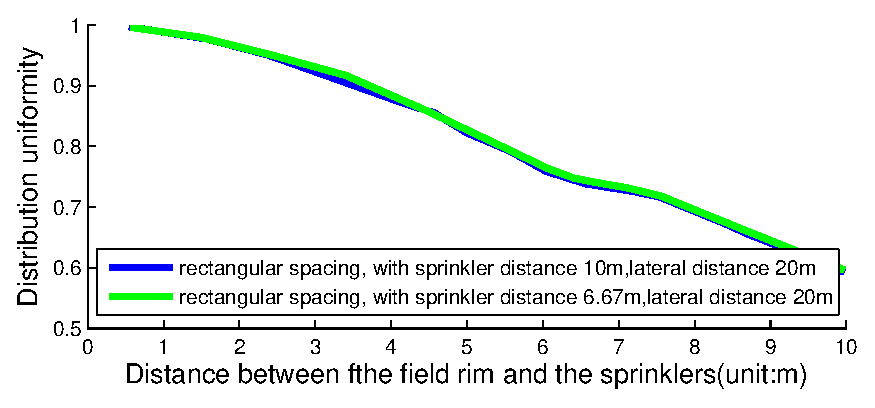
\includegraphics[width=0.8\textwidth]{fig11.eps} \caption{\label{fig11} $DU$ plotted vs. distance from the rim to the sprinkler
in 2 different situations }
\end{figure}


\subsubsection{Layout of the Pipe Set}

According to the analysis above, having 3 or 4 sprinklers along
the pipe only results in a slight difference. Considering that the
spraying radius (19m) is too large compared with the sprinkler
distance 6.67m when having 4 sprinklers, we choose to have 3. Thus
the only two feasible layouts of the whole system
exist\footnote{We are not considering the situation when the pipes
are not parallel to the edge of the field, because layout of this
kind is not practical.} (Figure 12 and Figure 13). Simply
speaking, Layout 1 implies that it requires 5 times of moving and
setting up the pipes while Layout 2 requires 6. But it's too early
to judge which is better.

\begin{figure}[!htb]
\centering
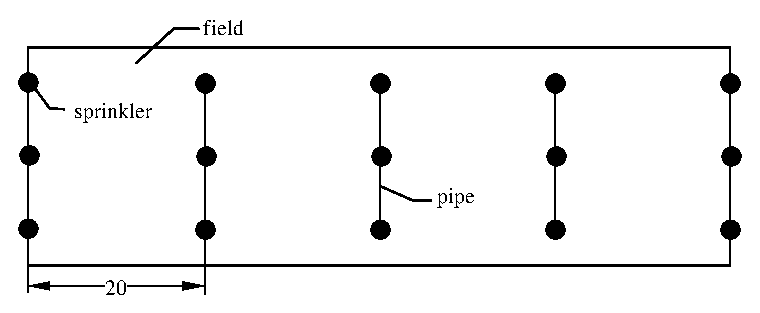
\includegraphics[width=0.8\textwidth]{fig12.eps} \caption{\label{fig12} Layout 1. }
\end{figure}

\begin{figure}[!htb]
\centering
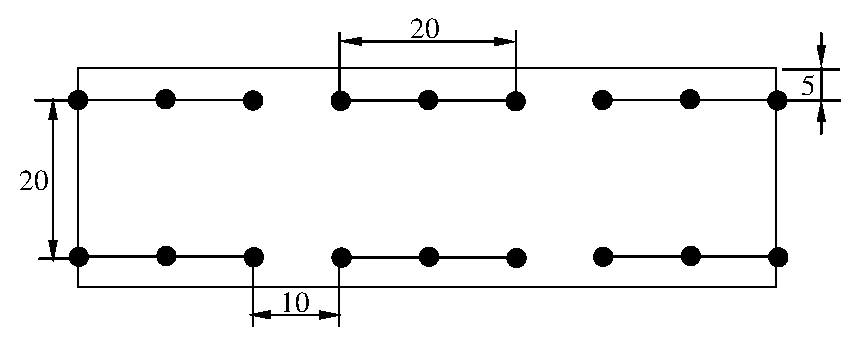
\includegraphics[width=0.92\textwidth]{fig13.eps} \caption{\label{fig13} Layout 2. }
\end{figure}

For further estimation, we should calculate $DU$ (Distribution
Uniformity) of both layouts. The result from the simulation of
catch-can tests is shown in following figures:

\newpage

\begin{figure}[!htb]
\centering
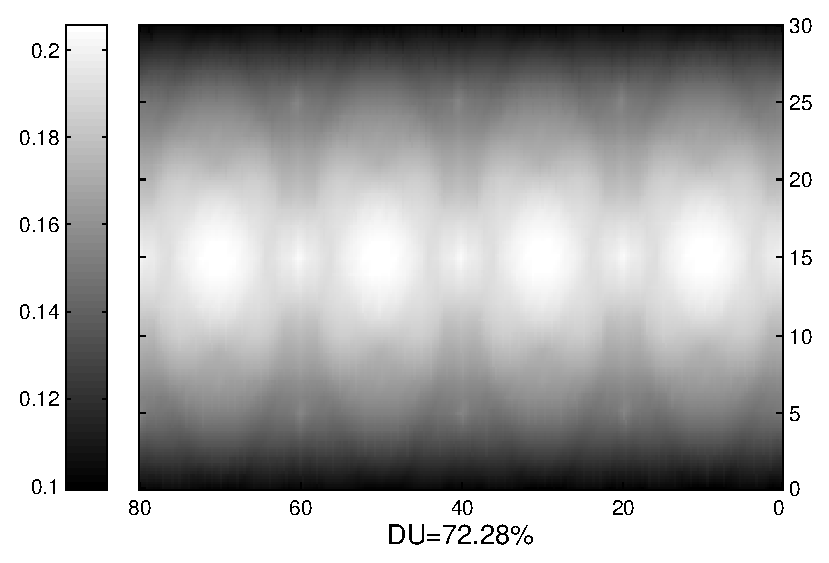
\includegraphics[width=0.8\textwidth]{fig14.eps} \caption{\label{fig14} Catch-can test simulation result of layout 1. }
\end{figure}


\begin{figure}[!htb]
\centering
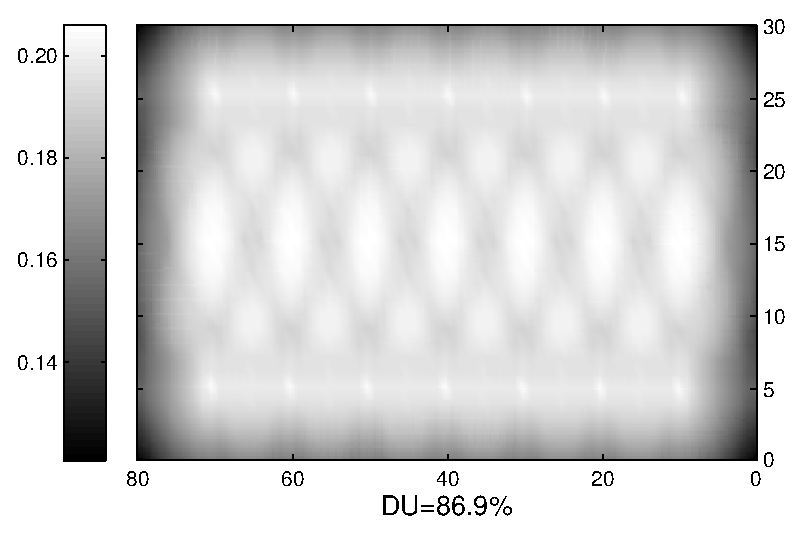
\includegraphics[width=0.8\textwidth]{fig15.eps} \caption{\label{fig15} Catch-can test simulation result of Layout 2. }
\end{figure}

We decide to abandon Layout 1 because it has a very poor DU. After
slightly changing the lateral distance in Layout 2, we finally
achieve a best DU of 89.5\% in Layout 3 (see in Figure 16):
\newpage

\begin{figure}[!htb]
\centering
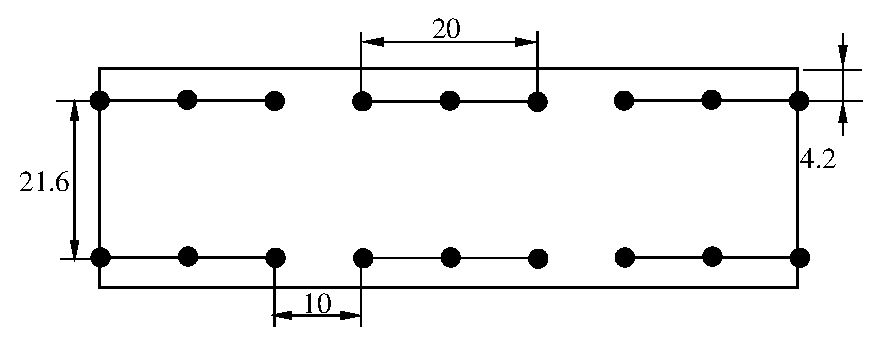
\includegraphics[width=0.8\textwidth]{fig161.eps}
\end{figure}

\begin{figure}[!htb]
\centering
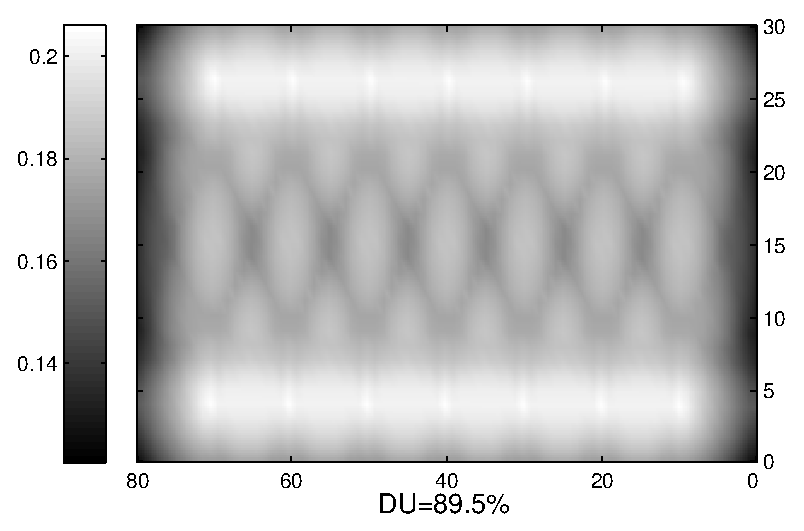
\includegraphics[width=0.8\textwidth]{fig162.eps}
\caption{\label{fig16} Upper: Layout3; Lower: Catch-can test
simulation result of Layout 3. }
\end{figure}

Then, if we are brave enough to move some sprinklers out of the
field, we'll achieve a higher $DU$ in Layout 4 (see in Figure 17):
\newpage

\begin{figure}[!htb]
\centering
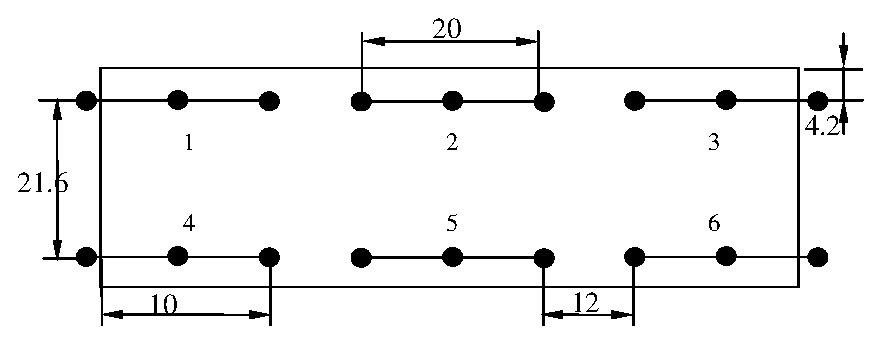
\includegraphics[width=0.8\textwidth]{fig171.eps}
\end{figure}

\begin{figure}[!htb]
\centering
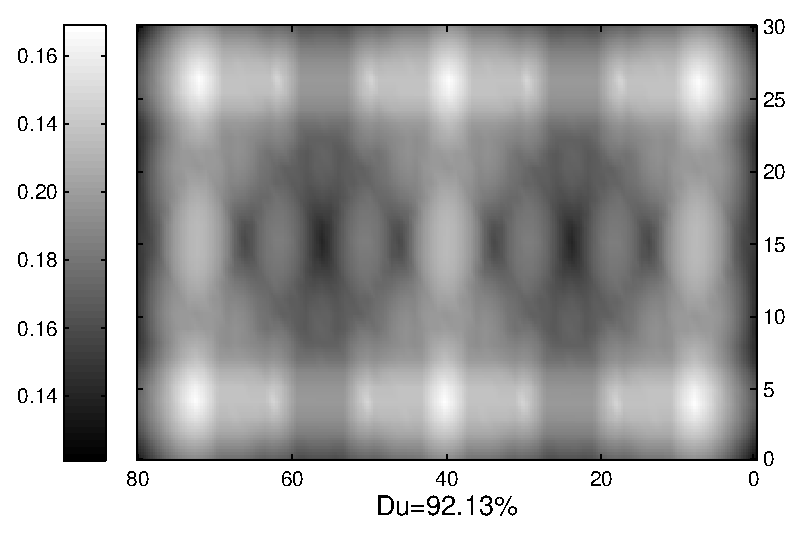
\includegraphics[width=0.8\textwidth]{fig172.eps}
\caption{\label{fig17} Upper: Layout4; Lower: Catch-can test
simulation result of Layout }
\end{figure}

\subsubsection{Calculation of the Precipitation}

In order to meet the problem's constraints that in any part of the
field,

\begin{description}
\item[a)] the precipitation rate $\geq 2 cm/4 days\ldots\ldots$(Constraint A),

\item[b)] the precipitation rate $\leq0.75 cm/hour\ldots\ldots$(Constraint B),
\end{description}

we should calculate the precipitation rate of the system in Layout
4 before scheduling the interval to irrigating the field and to
move the pipe.

\begin{figure}[!htb]
\centering
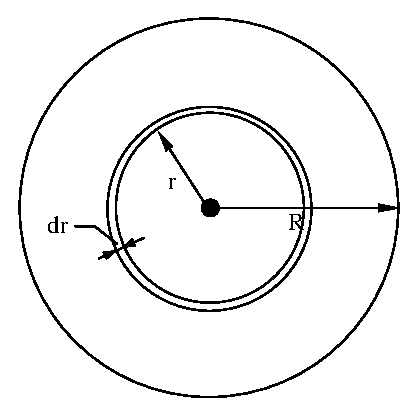
\includegraphics[width=0.4\textwidth]{fig18.eps}
\caption{\label{fig18} Precipitation area of a single sprinkler.}
\end{figure}

The precipitation area of a sprinkler should be a circle with a
radius $R$, as Figure 18 shows. The profile of the precipitation
rate distribution is in Figure 5. In order to figure out the
precipitation rate at a certain point whose distance from the
sprinkler is $r$, we firstly calculate the angle $\alpha$ in
Figure 5. As we normalize the distribution, we get

\[
\int_0^R(R-r)\tan\alpha\cdot2\pi r \textrm{d}r
\]

so

\[
\tan\alpha=\frac{3}{\pi R^3}
\]

then the precipitation rate

\[
pr(r)=v(R-r)\tan\alpha=\frac{3(R-r)}{\pi R^3}v,
\]

where $R=19m$, $v=50lpm$.

With Matlab, we calculated the precipitation rate at each point in
the $80m\times30m$ field, with the irrigation system working only
once (see in Figure 19 Right) and after a complete cycle of moving
the equipment and irrigating (see in Figure 19 Left).

\begin{figure}[!htb]
\centering
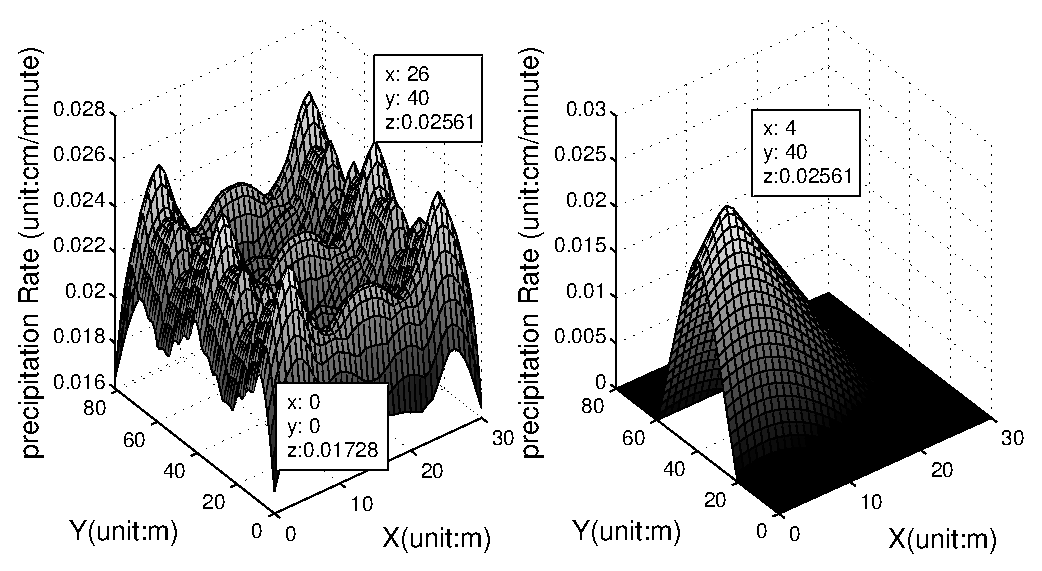
\includegraphics[width=1\textwidth]{fig19.eps}
\caption{\label{fig19} Precipitation rate of water in the field
with Layout 4. Left: the whole effect of 6 pipes together; Right:
the effect of a 20m pipe working alone.}
\end{figure}

\subsubsection{Scheduling the Irrigation Time}

Figure 19 Right shows that when the sprinklers (only one $20m$
pipe at a time) are working, the maximum precipitation rate is

\[
0.02561cm/min.
\]

To satisfy Constraint A, the period of irrigation should be less
than

\[
\frac{0.75cm/hour}{0.02561cm/min}=29.30\textrm{min per hour}
\]

Because the smaller the period of irrigation is, the more
frequently the farmer should stop to move the pipe, we thus choose
a large but easy to implement one:

\[
25 \textrm{min per hour.}
\]

Figure 19 Left shows that after a complete cycle of irrigation the
whole field, i.e. the equipment has been moved to and irrigated
every required place of the field, and the minimum precipitation
rate is

\[
0.01728 cm/min
\]

To satisfy Constraint B, the period of irrigation should be longer
than

\[
\frac{2cm/4days}{0.01728cm/min}=115.7\textrm{min every 4 days}
\]

To meet this, in every 4 days, we plan to irrigate the same place
5 times, every time lasts 25 minutes, that is 125 minutes, well
satisfies Constraint B.

With the same method, we calculate the same parameters for Layout
3, and list the comparison in Table 6:

\begin{table}[!htb]
\centering \caption{Comparison between Layout 3 and Layout 4.}
\begin{tabular}{l|ll}
\hline
\multicolumn{1}{c|}{} & \multicolumn{1}{c}{Layout 3} & \multicolumn{1}{c}{Layout 4} \\
\hline
\multicolumn{1}{c|}{Max precipitation rate (cm/min)} & \multicolumn{1}{c}{0.02561} & \multicolumn{1}{c}{0.02561} \\
\hline
\multicolumn{1}{c|}{Min precipitation rate (cm/min)} & \multicolumn{1}{c}{0.01598} & \multicolumn{1}{c}{0.01728} \\
\multicolumn{1}{c|}{Total Irrigation time every 4 days } & \multicolumn{1}{c}{$150\times6$} & \multicolumn{1}{c}{$125\times6$} \\
\multicolumn{1}{c|}{(min)} & \multicolumn{1}{c}{} & \multicolumn{1}{c}{} \\
\multicolumn{1}{c|}{DU, Distribution Uniformity} & \multicolumn{1}{c}{89.5\%} & \multicolumn{1}{c}{92.1\%} \\
\hline
\end{tabular}
\end{table}

It is clearly shown that Layout 4 not only has higher DU than
Layout 3, but also saves 16.7\% of water, in other words, has
higher application efficiency, though one of its sprinklers is
positioned out of the field in some situation. This is because
that Layout 3 has a smaller min precipitation rate which leads to
more irrigation time in order to satisfy Constraint A. So we
choose Layout 4 as our solution.


\subsection{Stage3: Schedule Design}


 As we've discussed in the previous stage, our schedules will be able to achieve a DU as high as 92.1\% after a cycle of 4-day-irrigation. We have two concrete design of irrigation timetable.

The first design make the least moving time but, to some extent,
is not so "average" as it gathers sprinkling processes of the same
sprinkler together. (Table 7)

\begin{table}[!htb]
\centering \caption{The first schedule for every four days.('$^*$'
means it is required to set up the pipe set in the referred
position before irrigation. And the position code refers to pipe's
position in Figure 17)}
\begin{tabular}{lllll}
\hline
\multicolumn{1}{c}{Day} & \multicolumn{1}{c}{} & \multicolumn{1}{c}{Time} & \multicolumn{1}{c}{} & \multicolumn{1}{c}{Position code} \\
\hline
\multicolumn{1}{c}{1} & \multicolumn{1}{c}{} & \multicolumn{1}{r}{7:00-7:25} & \multicolumn{1}{r}{} & \multicolumn{1}{c}{$1^*$} \\
\multicolumn{1}{c}{} & \multicolumn{1}{c}{} & \multicolumn{1}{r}{8:00-8:25} & \multicolumn{1}{r}{} & \multicolumn{1}{c}{1} \\
\multicolumn{1}{c}{} & \multicolumn{1}{c}{} & \multicolumn{1}{r}{9:00-9:25} & \multicolumn{1}{r}{} & \multicolumn{1}{c}{1} \\
\multicolumn{1}{c}{} & \multicolumn{1}{c}{} & \multicolumn{1}{r}{10:00-10:25} & \multicolumn{1}{r}{} & \multicolumn{1}{c}{1} \\
\multicolumn{1}{c}{} & \multicolumn{1}{c}{} & \multicolumn{1}{r}{11:00-11:25} & \multicolumn{1}{r}{} & \multicolumn{1}{c}{1} \\
\multicolumn{1}{c}{} & \multicolumn{1}{c}{} & \multicolumn{1}{r}{13:00-13:25} & \multicolumn{1}{r}{} & \multicolumn{1}{c}{$6^*$} \\
\multicolumn{1}{c}{} & \multicolumn{1}{c}{} & \multicolumn{1}{r}{14:00-14:25} & \multicolumn{1}{r}{} & \multicolumn{1}{c}{6} \\
\multicolumn{1}{c}{} & \multicolumn{1}{c}{} & \multicolumn{1}{r}{15:00-15:25} & \multicolumn{1}{r}{} & \multicolumn{1}{c}{6} \\
\multicolumn{1}{c}{2} & \multicolumn{1}{c}{} & \multicolumn{1}{r}{7:00-7:25} & \multicolumn{1}{r}{} & \multicolumn{1}{c}{6} \\
\multicolumn{1}{c}{} & \multicolumn{1}{c}{} & \multicolumn{1}{r}{8:00-8:25} & \multicolumn{1}{r}{} & \multicolumn{1}{c}{6} \\
\multicolumn{1}{c}{} & \multicolumn{1}{c}{} & \multicolumn{1}{r}{9:00-9:25} & \multicolumn{1}{r}{} & \multicolumn{1}{c}{$2^*$} \\
\multicolumn{1}{c}{} & \multicolumn{1}{c}{} & \multicolumn{1}{r}{10:00-10:25} & \multicolumn{1}{r}{} & \multicolumn{1}{c}{2} \\
\multicolumn{1}{c}{} & \multicolumn{1}{c}{} & \multicolumn{1}{r}{11:00-11:25} & \multicolumn{1}{r}{} & \multicolumn{1}{c}{2} \\
\multicolumn{1}{c}{} & \multicolumn{1}{c}{} & \multicolumn{1}{r}{13:00-13:25} & \multicolumn{1}{r}{} & \multicolumn{1}{c}{2} \\
\multicolumn{1}{c}{} & \multicolumn{1}{c}{} & \multicolumn{1}{r}{14:00-14:25} & \multicolumn{1}{r}{} & \multicolumn{1}{c}{2} \\
\multicolumn{1}{c}{} & \multicolumn{1}{c}{} & \multicolumn{1}{r}{15:00-15:25} & \multicolumn{1}{r}{} & \multicolumn{1}{c}{$4^*$} \\
\multicolumn{1}{c}{3} & \multicolumn{1}{c}{} & \multicolumn{1}{r}{7:00-7:25} & \multicolumn{1}{r}{} & \multicolumn{1}{c}{4} \\
\multicolumn{1}{c}{} & \multicolumn{1}{c}{} & \multicolumn{1}{r}{8:00-8:25} & \multicolumn{1}{r}{} & \multicolumn{1}{c}{4} \\
\multicolumn{1}{c}{} & \multicolumn{1}{c}{} & \multicolumn{1}{r}{9:00-9:25} & \multicolumn{1}{r}{} & \multicolumn{1}{c}{4} \\
\multicolumn{1}{c}{} & \multicolumn{1}{c}{} & \multicolumn{1}{r}{10:00-10:25} & \multicolumn{1}{r}{} & \multicolumn{1}{c}{4} \\
\multicolumn{1}{c}{} & \multicolumn{1}{c}{} & \multicolumn{1}{r}{11:00-11:25} & \multicolumn{1}{r}{} & \multicolumn{1}{c}{$3^*$} \\
\multicolumn{1}{c}{} & \multicolumn{1}{c}{} & \multicolumn{1}{r}{13:00-13:25} & \multicolumn{1}{r}{} & \multicolumn{1}{c}{3} \\
\multicolumn{1}{c}{} & \multicolumn{1}{c}{} & \multicolumn{1}{r}{14:00-14:25} & \multicolumn{1}{r}{} & \multicolumn{1}{c}{3} \\
\multicolumn{1}{c}{4} & \multicolumn{1}{c}{} & \multicolumn{1}{r}{7:00-7:25} & \multicolumn{1}{r}{} & \multicolumn{1}{c}{3} \\
\multicolumn{1}{c}{} & \multicolumn{1}{c}{} & \multicolumn{1}{r}{8:00-8:25} & \multicolumn{1}{r}{} & \multicolumn{1}{c}{3} \\
\multicolumn{1}{c}{} & \multicolumn{1}{c}{} & \multicolumn{1}{r}{9:00-9:25} & \multicolumn{1}{r}{} & \multicolumn{1}{c}{$5^*$} \\
\multicolumn{1}{c}{} & \multicolumn{1}{c}{} & \multicolumn{1}{r}{10:00-10:25} & \multicolumn{1}{r}{} & \multicolumn{1}{c}{5} \\
\multicolumn{1}{c}{} & \multicolumn{1}{c}{} & \multicolumn{1}{r}{11:00-11:25} & \multicolumn{1}{r}{} & \multicolumn{1}{c}{5} \\
\multicolumn{1}{c}{} & \multicolumn{1}{c}{} & \multicolumn{1}{r}{13:00-13:25} & \multicolumn{1}{r}{} & \multicolumn{1}{c}{5} \\
\multicolumn{1}{c}{} & \multicolumn{1}{c}{} & \multicolumn{1}{r}{14:00-14:25} & \multicolumn{1}{r}{} & \multicolumn{1}{c}{5} \\
\hline

\end{tabular}

\end{table}




The second design need more moving time but, as a kind of
compensation, is more "average" (for instance, the field receives
water much more evenly in time) than the first design. (Table 8)


\begin{table}[!htb]
\centering \caption{The second schedule for every four days.}

(position code refers to Figure 16)


\begin{tabular}{lllll}
\hline
\multicolumn{1}{c}{Day} & \multicolumn{1}{c}{} & \multicolumn{1}{c}{Time} & \multicolumn{1}{c}{} & \multicolumn{1}{c}{Position code} \\
\hline
\multicolumn{1}{c}{1} & \multicolumn{1}{c}{} & \multicolumn{1}{r}{7:00-7:25} & \multicolumn{1}{r}{} & \multicolumn{1}{c}{1} \\
\multicolumn{1}{c}{} & \multicolumn{1}{c}{} & \multicolumn{1}{r}{8:00-8:25} & \multicolumn{1}{r}{} & \multicolumn{1}{c}{5} \\
\multicolumn{1}{c}{} & \multicolumn{1}{c}{} & \multicolumn{1}{r}{9:00-9:25} & \multicolumn{1}{r}{} & \multicolumn{1}{c}{3} \\
\multicolumn{1}{c}{} & \multicolumn{1}{c}{} & \multicolumn{1}{r}{10:00-10:25} & \multicolumn{1}{r}{} & \multicolumn{1}{c}{4} \\
\multicolumn{1}{c}{} & \multicolumn{1}{c}{} & \multicolumn{1}{r}{11:00-11:25} & \multicolumn{1}{r}{} & \multicolumn{1}{c}{2} \\
\multicolumn{1}{c}{} & \multicolumn{1}{c}{} & \multicolumn{1}{r}{13:00-13:25} & \multicolumn{1}{r}{} & \multicolumn{1}{c}{6} \\
\multicolumn{1}{c}{} & \multicolumn{1}{c}{} & \multicolumn{1}{r}{14:00-14:25} & \multicolumn{1}{r}{} & \multicolumn{1}{c}{1} \\
\multicolumn{1}{c}{} & \multicolumn{1}{c}{} & \multicolumn{1}{r}{15:00-15:25} & \multicolumn{1}{r}{} & \multicolumn{1}{c}{5} \\
\multicolumn{1}{c}{2} & \multicolumn{1}{c}{} & \multicolumn{1}{r}{7:00-7:25} & \multicolumn{1}{r}{} & \multicolumn{1}{c}{3} \\
\multicolumn{1}{c}{} & \multicolumn{1}{c}{} & \multicolumn{1}{r}{8:00-8:25} & \multicolumn{1}{r}{} & \multicolumn{1}{c}{4} \\
\multicolumn{1}{c}{} & \multicolumn{1}{c}{} & \multicolumn{1}{r}{9:00-9:25} & \multicolumn{1}{r}{} & \multicolumn{1}{c}{2} \\
\multicolumn{1}{c}{} & \multicolumn{1}{c}{} & \multicolumn{1}{r}{10:00-10:25} & \multicolumn{1}{r}{} & \multicolumn{1}{c}{6} \\
\multicolumn{1}{c}{} & \multicolumn{1}{c}{} & \multicolumn{1}{r}{11:00-11:25} & \multicolumn{1}{r}{} & \multicolumn{1}{c}{1} \\
\multicolumn{1}{c}{} & \multicolumn{1}{c}{} & \multicolumn{1}{r}{13:00-13:25} & \multicolumn{1}{r}{} & \multicolumn{1}{c}{5} \\
\multicolumn{1}{c}{} & \multicolumn{1}{c}{} & \multicolumn{1}{r}{14:00-14:25} & \multicolumn{1}{r}{} & \multicolumn{1}{c}{3} \\
\multicolumn{1}{c}{} & \multicolumn{1}{c}{} & \multicolumn{1}{r}{15:00-15:25} & \multicolumn{1}{r}{} & \multicolumn{1}{c}{4} \\
\multicolumn{1}{c}{3} & \multicolumn{1}{c}{} & \multicolumn{1}{r}{7:00-7:25} & \multicolumn{1}{r}{} & \multicolumn{1}{c}{2} \\
\multicolumn{1}{c}{} & \multicolumn{1}{c}{} & \multicolumn{1}{r}{8:00-8:25} & \multicolumn{1}{r}{} & \multicolumn{1}{c}{6} \\
\multicolumn{1}{c}{} & \multicolumn{1}{c}{} & \multicolumn{1}{r}{9:00-9:25} & \multicolumn{1}{r}{} & \multicolumn{1}{c}{1} \\
\multicolumn{1}{c}{} & \multicolumn{1}{c}{} & \multicolumn{1}{r}{10:00-10:25} & \multicolumn{1}{r}{} & \multicolumn{1}{c}{5} \\
\multicolumn{1}{c}{} & \multicolumn{1}{c}{} & \multicolumn{1}{r}{11:00-11:25} & \multicolumn{1}{r}{} & \multicolumn{1}{c}{3} \\
\multicolumn{1}{c}{} & \multicolumn{1}{c}{} & \multicolumn{1}{r}{13:00-13:25} & \multicolumn{1}{r}{} & \multicolumn{1}{c}{4} \\
\multicolumn{1}{c}{} & \multicolumn{1}{c}{} & \multicolumn{1}{r}{14:00-14:25} & \multicolumn{1}{r}{} & \multicolumn{1}{c}{2} \\
\multicolumn{1}{c}{4} & \multicolumn{1}{c}{} & \multicolumn{1}{r}{7:00-7:25} & \multicolumn{1}{r}{} & \multicolumn{1}{c}{6} \\
\multicolumn{1}{c}{} & \multicolumn{1}{c}{} & \multicolumn{1}{r}{8:00-8:25} & \multicolumn{1}{r}{} & \multicolumn{1}{c}{1} \\
\multicolumn{1}{c}{} & \multicolumn{1}{c}{} & \multicolumn{1}{r}{9:00-9:25} & \multicolumn{1}{r}{} & \multicolumn{1}{c}{5} \\
\multicolumn{1}{c}{} & \multicolumn{1}{c}{} & \multicolumn{1}{r}{10:00-10:25} & \multicolumn{1}{r}{} & \multicolumn{1}{c}{3} \\
\multicolumn{1}{c}{} & \multicolumn{1}{c}{} & \multicolumn{1}{r}{11:00-11:25} & \multicolumn{1}{r}{} & \multicolumn{1}{c}{4} \\
\multicolumn{1}{c}{} & \multicolumn{1}{c}{} & \multicolumn{1}{r}{13:00-13:25} & \multicolumn{1}{r}{} & \multicolumn{1}{c}{2} \\
\multicolumn{1}{c}{} & \multicolumn{1}{c}{} & \multicolumn{1}{r}{14:00-14:25} & \multicolumn{1}{r}{} & \multicolumn{1}{c}{6} \\
\hline
\end{tabular}
\end{table}

\section{Evaluation of Results}

\subsection{Comparison between Two Designs}

\begin{table}[!htb] \centering \caption{Comparison between Design 1 and Design 2.}
\begin{tabular}{lll}
\hline
\multicolumn{1}{c}{Parameters in one cycle of irrigation (4days) } & \multicolumn{1}{c}{Design 1} & \multicolumn{1}{c}{Design 2} \\
\hline
\multicolumn{1}{c}{Number of equipment resets } & \multicolumn{1}{c}{6} & \multicolumn{1}{c}{30} \\
\multicolumn{1}{c}{Equipment reset time (one reset cost} & \multicolumn{1}{c}{} & \multicolumn{1}{c}{} \\
\multicolumn{1}{c}{ 30min as assumed) (hour)} & \multicolumn{1}{c}{3} & \multicolumn{1}{c}{15} \\
\multicolumn{1}{c}{Irrigation time (hour)} & \multicolumn{1}{c}{12.5} & \multicolumn{1}{c}{12.5} \\
\multicolumn{1}{c}{DU, Distribution Uniformity} & \multicolumn{1}{c}{92.1\%} & \multicolumn{1}{c}{92.1\%} \\
\hline
\end{tabular}
\end{table}

Actually, Design 1 is the most time effective and labor saving
schedule based on Layout 4. If the water source, i.e. the pump,
has a timing mechanism (there is such product in market), the
whole irrigation only costs 3 hours labor time every 4 days. But
as we've discussed, Design 2 has a more "average" irrigation,
which may be better for crops or plants. So it is easy to arrange
a more compromising schedule good for plants and with longer but
acceptable required labor time.

It is also worthy mentioning that with the sector mechanism, we
can control the rotating range of the sprinkler on the edge of or
out of the field to reduce the water waste.

\section{Strengths and Weaknesses}

\subsection{Strengths}
\begin{itemize}
\item We use real data of sprinklers to determine the parameters of the sprinklers we choose and determine the number of sprinklers.

\item We establish a model based on the engineering knowledge of sprinklers, and find out the overall precipitation distribution, and then manage to find out an optimal schedule. All the results are based on calculations.

\item Our model to analyze the layout of the irrigation system is sprinkler-independent. This means, for whatever kind of sprinkler, if its single precipitation profile is known (e.g. though a real catch-can test), we can determine the precipitation profile across the whole field.

\item The placement and schedule is very clear and easy to implement.
\end{itemize}

\subsection{Weaknesses}
\begin{itemize}
\item Water pressure in the pipe may diverse, and so the discharge of the sprinklers may not be exactly the same.
\end{itemize}

\section{Further Discussion}

The analysis should further include the consideration of wind,
evaporation, the characters of the soil type and penetration.

\newpage
\begin{thebibliography}{1}
\bibitem{1}Wikipedia, the free encyclopedia - entry: Bernoulli's equation,
http://en.wikipedia.org/wiki/Bernoulli\%27s\_equation

\bibitem{1}Handbook of sprinkling irrigation engineering, Water Resources
and Electric Power Press,1989:p.32-36,40-42,44

\bibitem{1}Gary P. Merkley , Richard G. Allen, Sprinkle and Trickle
Irrigation Lecture Notes, Utah State University, Fall Semester
2004,
\\http://www.irri-net.org/documents/sprinkle\%20and\%20trickle\%20irrigation.pdf:p.25-27,29,40

\bibitem{1}RainBird - Distribution Uniformity for Sprinkler Irrigation
\\http://www.rainbird.com/ag/du.htm
\end{thebibliography}

\end{document}
